\subsection{User Interfaces}
This section shows a mockup version of the main functionalities of the mobile application and the web application of the final version of SafeStreets.
\begin{itemize}
    \item \textit{Mobile application}:
            \begin{figure}[H]
                \centering
                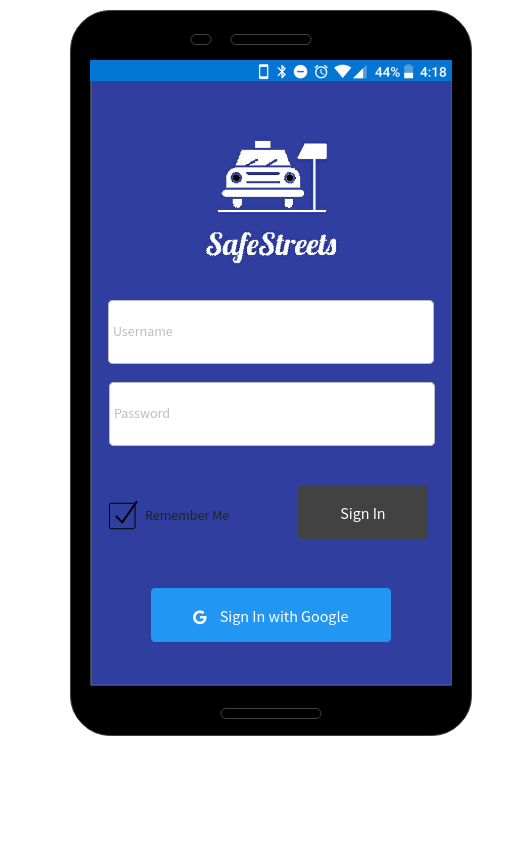
\includegraphics[width=0.40\textwidth]{login_app}
                \caption{LogIn interface}
                \label{fig:login_app}
            \end{figure}
            The Figure \ref{fig:login_app} represents the login form of the SafeStreets
            mobile application. The user can login through his username
            and password, or his Google account.
            \begin{figure}[H]
                \centering
                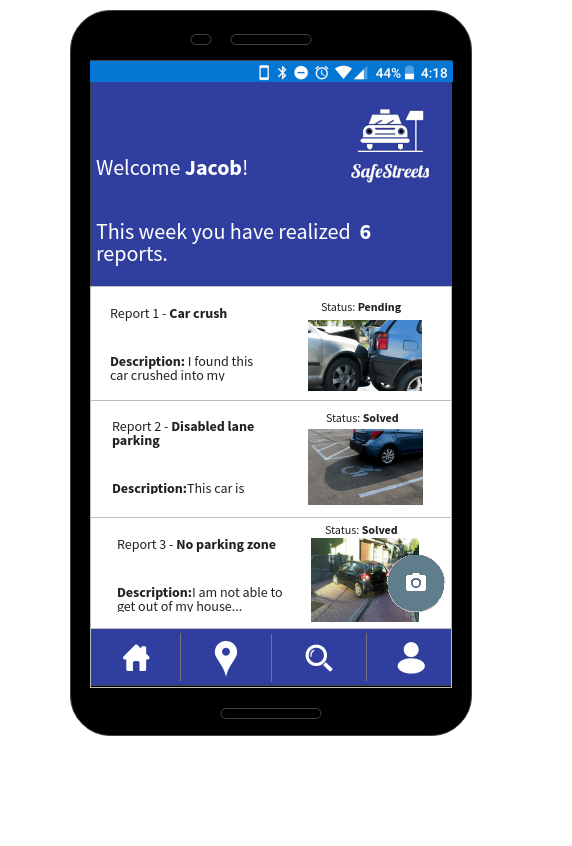
\includegraphics[width=0.45\textwidth]{home_app}
                \caption{Homepage}
                \label{fig:home_app}
            \end{figure}
            The figure \ref{fig:home_app} represents the homepage of the SafeStreets
            mobile application. The user is allowed to look at the list
            of the violation reports that he published, publish a new one
            through the floating button or visit other sections of the app.
            \begin{figure}[H]
                \centering
                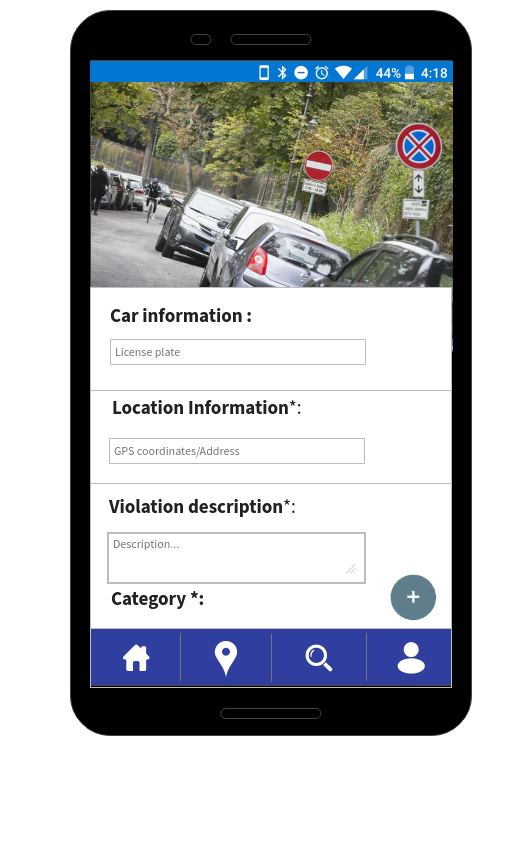
\includegraphics[width=0.45\textwidth]{violations_app}
                \caption{Violation report publishing page}
                \label{fig:violations_app}
            \end{figure}
            The figure \ref{fig:violations_app} represents the violations report
            publishing page of the SafeStreets mobile application. 
            The user is allowed take a picture of the violation clicking on the camera
            button and fill in the form to realize the violation report.
            \begin{figure}[H]
                \centering
                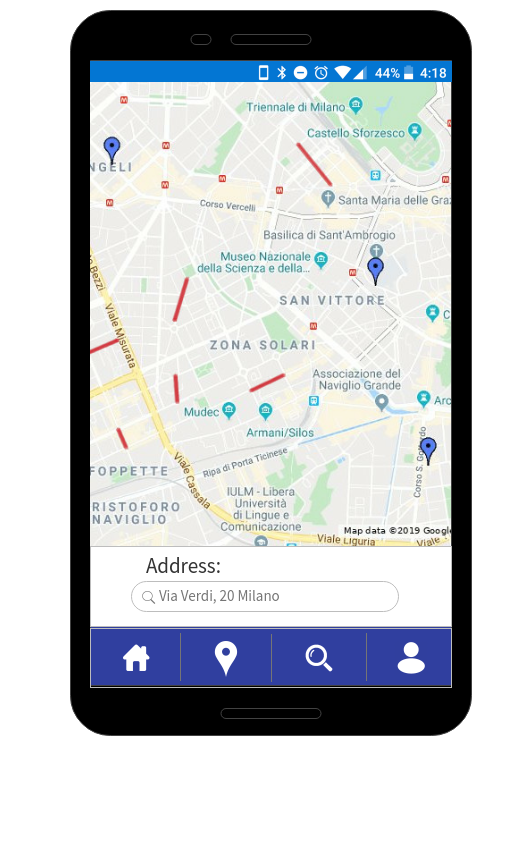
\includegraphics[width=0.45\textwidth]{maps_app}
                \caption{Map search page}
                \label{fig:maps_app}
            \end{figure}
            The figure \ref{fig:maps_app} represents the map page of the SafeStreets mobile application. 
            The user is allowed to look at the MDS highlighted in red on the map. It is also
            possible to search for a specific address through the search bar.
            \newpage
    \item  \textit{Web application}:
    \begin{figure}[H]
        \centering
        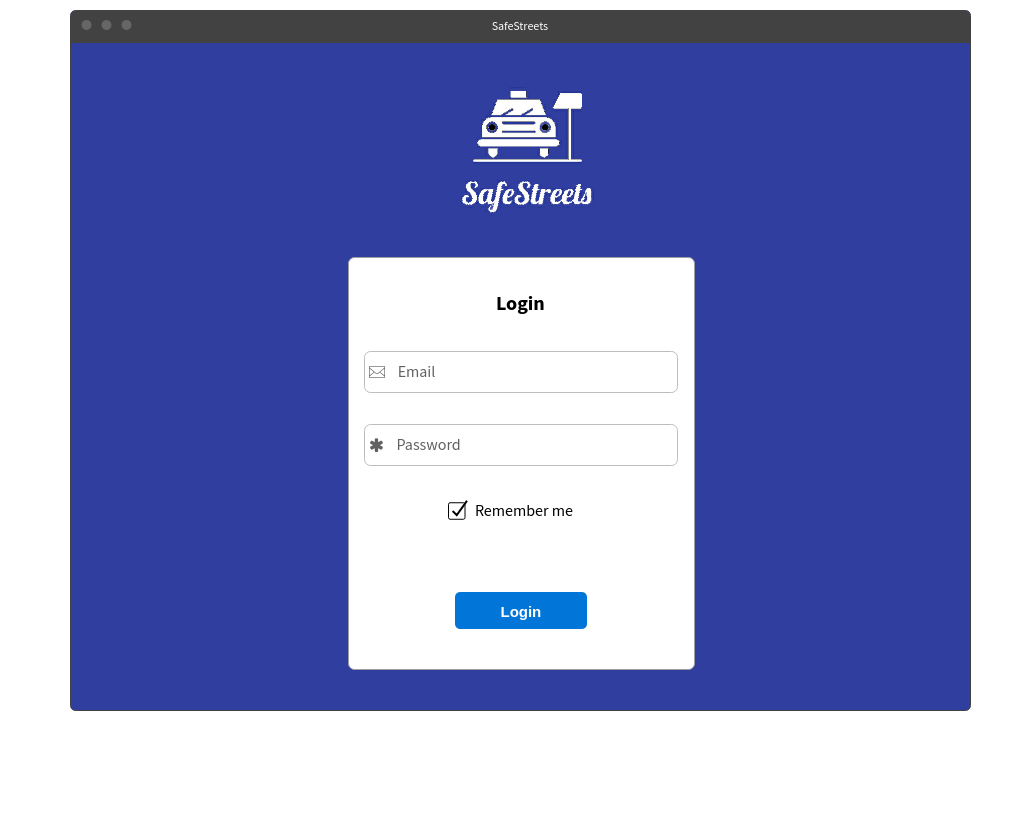
\includegraphics[width=0.75\textwidth]{login_web}
        \caption{LogIn interface}
        \label{fig:login_web}
    \end{figure}
    The Figure \ref{fig:login_web} represents the login form of the SafeStreets
    web application. The officer can login through his username
    and password.
    \begin{figure}[H]
        \centering
        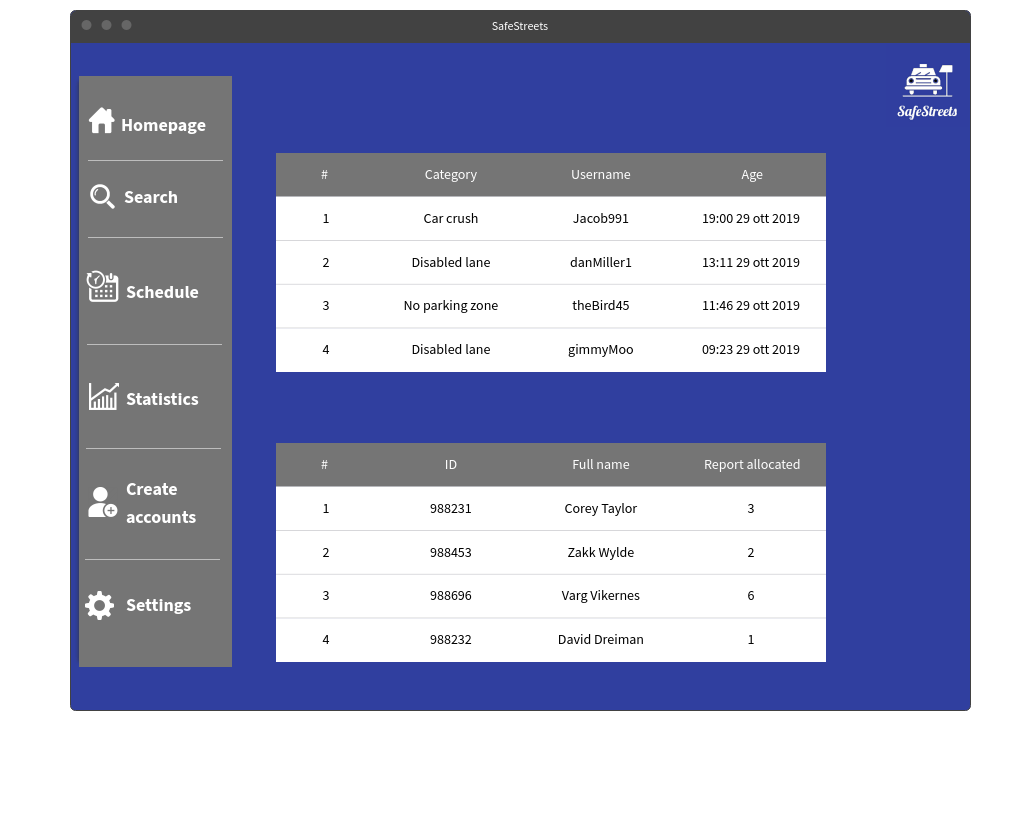
\includegraphics[width=0.75\textwidth]{home_web}
        \caption{Homepage}
        \label{fig:home_web}
    \end{figure}
    The figure \ref{fig:home_web} represents the homepage of the SafeStreets
    web application. The local system administrator is able to look at the list
    of recent violations, the list of the registered police technicians or to visit
    other pages by the side menu.
    \begin{figure}[H]
        \centering
        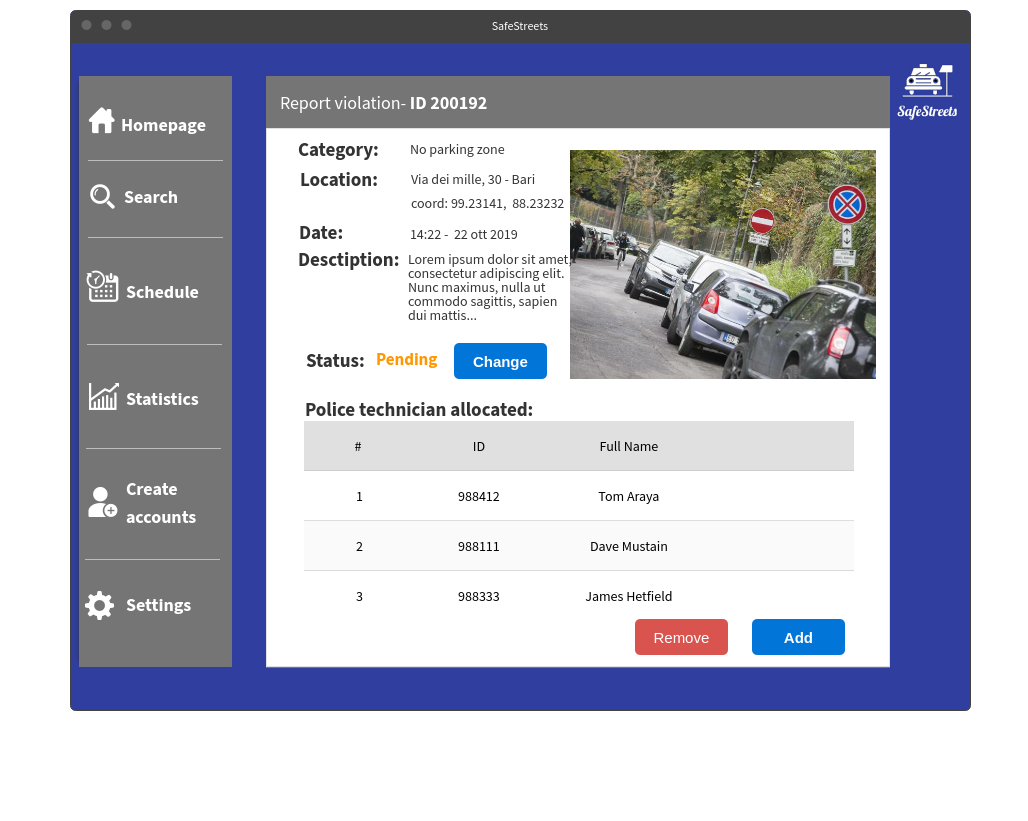
\includegraphics[width=0.75\textwidth]{report_web}
        \caption{Specific violation report page}
        \label{fig:report_web}
    \end{figure}
    The figure \ref{fig:report_web} represents the specific violations report
    page of the SafeStreets web application. 
    Both the LSA and the PT are able to look at the full violation report and they can change the report status from Pending to Closed (or viceversa). However, the LSA only can allocate/deallocate police technicians from this specific report.
    \begin{figure}[H]
        \centering
        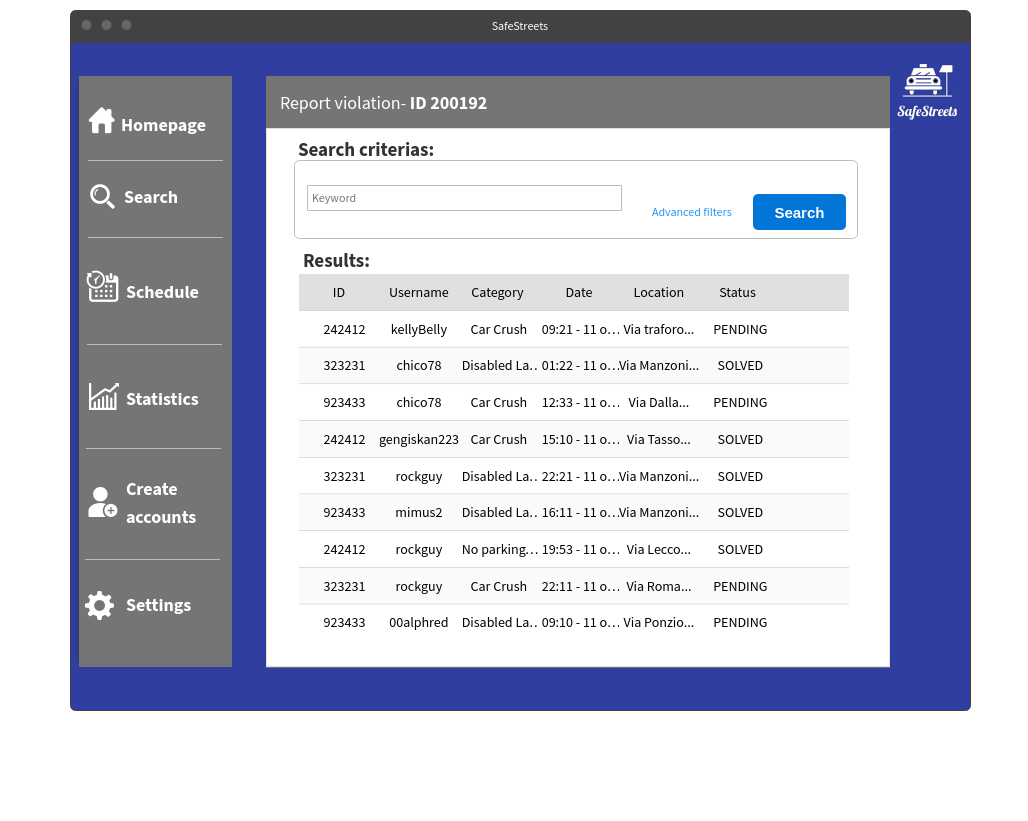
\includegraphics[width=0.7\textwidth]{mine_web}
        \caption{Report mining page}
        \label{fig:mine_web}
    \end{figure}
    The figure \ref{fig:mine_web} represents the report search page of the SafeStreets web application. 
    The local system administrator is able to search for a set of violation applying a keyword filtering
    and some advanced filters, such as date range or location.
\end{itemize}
\newpage
\subsection{Hardware Interfaces}
SafeStreets do not require any specific hardware device, 
thus there are no hardware interfaces to other existing systems.
\subsection{Software Interfaces}
SafeStreets is a standalone service and does not share any API to 
external systems. However, the system requires the interaction with the Image recognition service and with the municipality's legacy system to perform its tasks. Also, a map service is required in order to show the MDS positions on the mobile application.\newline
The software requires a standard format in order to retrieve car accident.
Such standard will be specified more in details in the DD.
\subsection{Communication Interfaces}
External services are not allowed to interact actively with SafeStreets, therefore the system does not offer any communication interface to external systems.
